\documentclass[11pt,a4paper]{article}
\usepackage[utf8]{inputenc}
\usepackage[T1]{fontenc}
\usepackage[margin=19mm]{geometry}
\usepackage{amsmath,graphicx,booktabs,array,longtable,caption}
\usepackage[hidelinks]{hyperref}
\setlength{\tabcolsep}{3pt}
\setlength{\parindent}{0pt}
\setlength{\parskip}{6pt}
\title{Payload mass and mounting height in a balancing robot}
\author{Michael Agbo}
\date{12 November 2026}
\begin{document}
\maketitle
\section*{Scope and main findings}
This Step 4 research supplement extends the existing planar balancing-robot model with a rigid, centred payload. It evaluates frozen nominal PID-type and LQR gains over 2,016 deterministic trials and 2,160 trials combining loading with noisy sensing. The 4,176 primary records are accompanied by a separate integration audit. This is an exploratory simulation study, not a hardware experiment, a held-out benchmark or a matched-tuning comparison of controller classes.

\textbf{Deterministic inventory: 1,008 trials per controller}
\begin{longtable}{p{0.252\linewidth}p{0.216\linewidth}p{0.216\linewidth}p{0.216\linewidth}}
\toprule
Controller & Recovered & Unsettled & Fallen \\ \midrule \endhead
PID & 625 & 187 & 196 \\
LQR & 743 & 0 & 265 \\
\bottomrule
\end{longtable}
The inventory equally weights the 21 distinct load configurations, each with 48 initial-tilt/force/torque conditions. It is not a deployment probability. Payload does not produce a uniform deterioration: the selected nominal high-mounted examples show smaller peak tilt with added mass. That finding depends on the geometry, frozen gains and disturbance definition. Mass, COM and inertia all change, and the push acts at the loaded-body COM, so this study does not isolate mass alone.

In the noisy subset, PID-type has 1,080 upright-but-unsettled trials. LQR has 1,026 upright-but-unsettled trials and 54 falls. No noisy trial satisfies the original final-one-second dwell requirement. Conditional tail RMS metrics therefore describe the remaining motion separately from recovery. The selected nominal noisy comparisons all survive the full 10 seconds.

\section*{1 Rigid payload model}
The original body has mass m0=1.2 kg, axle-to-COM distance l0=0.18 m and pitch inertia I0=0.012 kg m\textasciicircum{}2 about its own COM. A payload of mass mp is fixed on the body centreline, with COM distance h from the axle. Its rectangular dimensions are width w=0.08 m in the fore-aft direction, height b=0.06 m along the body and lateral depth 0.12 m. Density varies with the selected mass; dimensions stay fixed. The attachment is assumed massless and rigid. No payload is added or removed during a trial.

The combined mass M, COM distance L and COM pitch inertia I follow component mass weighting and the parallel-axis theorem [1]. For rotation about the lateral axle, payload depth does not enter its own pitch inertia Ip. No horizontal COM offset is introduced, so the upright equilibrium angle remains zero.

\begin{equation}M=m_0+m_p,\quad L=(m_0l_0+m_ph)/M,\quad I_p=m_p(w^2+b^2)/12\end{equation}
\begin{equation}I=I_0+m_0(l_0-L)^2+I_p+m_p(h-L)^2\end{equation}
The independent identity I + M L\textasciicircum{}2 = I0 + m0 l0\textasciicircum{}2 + Ip + mp h\textasciicircum{}2 verifies inertia about the axle. Substituting M, L and I into the existing nonlinear plant updates translational inertia, gravity, translation-pitch coupling and rotational inertia together. Zero payload returns the original parameter values exactly.

\clearpage
\section*{2 Experimental protocol}
Added masses are 0, 0.25, 0.50, 0.75, 1.00 and 1.50 kg. Nonzero masses use h=0.10, 0.18, 0.30 and 0.40 m. Zero mass is evaluated once, at the bookkeeping height 0.18 m, giving 21 unique loads. The deterministic grid combines initial tilts 0, 5, 10 and 15 deg; horizontal forces 0, 5, 10 and 20 N; and total motor-torque limits 0.2, 0.4 and 0.7 N m. There are 48 conditions per load and controller, hence 2,016 trials. Only nonnegative initial tilts and force directions are covered; opposite-direction disturbances remain untested here.

The sensing subset uses four loads: unloaded, 0.75 kg at 0.18 m, 0.75 kg at 0.40 m, and 1.50 kg at 0.40 m. Three physical scenarios retain the Step 3 definitions below. Each is evaluated with direct measurements at zero delay, Kalman-filtered measurements at zero delay, and Kalman-filtered measurements at 10 ms delay. Angle-noise SD is 0.5 deg and gyro-noise SD is 2 deg/s. Thirty seeds per combination produce 2,160 trials.

\textbf{Physical scenarios for the sensing subset}
\begin{longtable}{p{0.252\linewidth}p{0.216\linewidth}p{0.216\linewidth}p{0.216\linewidth}}
\toprule
Scenario & Initial tilt (deg) & Force (N) & Limit (N m) \\ \midrule \endhead
Nominal & 5 & 5 & 0.7 \\
Large push & 0 & 20 & 0.7 \\
Low torque & 0 & 5 & 0.2 \\
\bottomrule
\end{longtable}
Every run lasts at most 10 s. A nonzero force is held from 2.00 to 2.20 s. It acts horizontally at the combined loaded-body COM; its pitch moment is F L cos(theta). Thus the application point moves with COM as payload changes. This preserves the original COM-force convention, but is not equivalent to pushing a fixed chassis attachment. Base/wheel properties, gravity and drag are unchanged. Control and sensing run at 200 Hz; nominal plant integration uses one fourth-order Runge-Kutta step per control interval. Motor torque is saturated at the selected total two-motor limit.

Both original controllers and the Step 3 Kalman estimator are frozen. The estimator still processes tilt and angular rate only, with ideal but delayed position and velocity channels, fixed per-interval angular-acceleration SD 50 rad/s\textasciicircum{}2, and no delay prediction. True plant states are used only for physics, visualisation and evaluation. Matching seed 1001+104729*i, i=0..29, supplies paired innovations across controllers, loads and sensing profiles. The protocol was written before this sweep but uses previously explored scenarios; it is not preregistered or an independent generalisation test.

\section*{3 Outcomes and uncertainty}
A fall occurs when absolute true tilt reaches 45 deg at a control endpoint. Recovery requires a final continuous one-second dwell within absolute tilt 1 deg, position 0.03 m and speed 0.03 m/s, after the pulse ends; for zero-force cases the reference is t=0. Surviving runs that miss this criterion are unsettled. Persistent noise can prevent recovery under this strict rule even when posture remains bounded.

Final-second RMS tilt, position and speed use the 201 control samples from 9 to 10 s, including both endpoints. They are null for falls and are compared only in groups where every trial runs for 10 s. Peak tilt, displacement, saturation time and integrated squared torque use the available pre-termination record; different fall times therefore imply different horizons. Squared torque is a control-effort measure, not electrical energy. Wilson 95\% intervals apply only to noisy fixed-condition fall fractions. IQR bars describe seed variation and are not confidence intervals. Deterministic grid fractions carry no sampling intervals; shared seeds do not make observer or load groups independent.

\clearpage
\section*{4 How the mass distribution changes}
\begin{figure}[htbp]
\centering
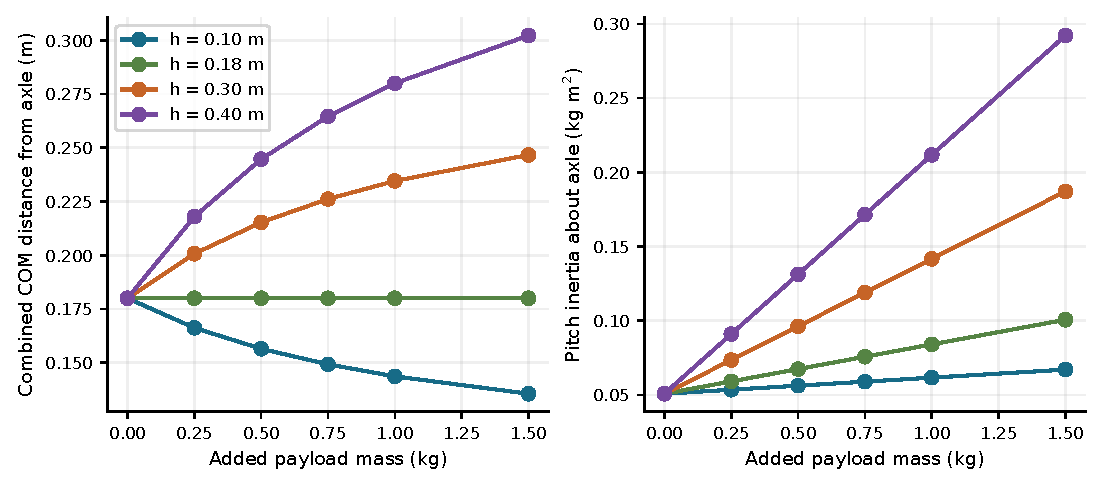
\includegraphics[width=\linewidth,height=.65\textheight,keepaspectratio]{../../figures/step4_fig01_mass_properties.pdf}
\caption{Rigid-body aggregation across the evaluated payload masses and mounting heights h. COM is measured along the body from the axle. The payload is a centred cuboid, 0.08 x 0.06 x 0.12 m; its own pitch inertia is included. Curves connect evaluated masses. The unloaded robot is the same at every nominal mounting height.}
\end{figure}
Moving a fixed mass above or below the original COM shifts the combined COM in the expected direction. Axle inertia increases for every positive added mass, while the rate of increase depends strongly on mounting height. These simultaneous changes explain why added load cannot be represented by changing body\_mass alone.

\clearpage
\section*{5 Loaded-body geometry in three dimensions}
\begin{figure}[htbp]
\centering
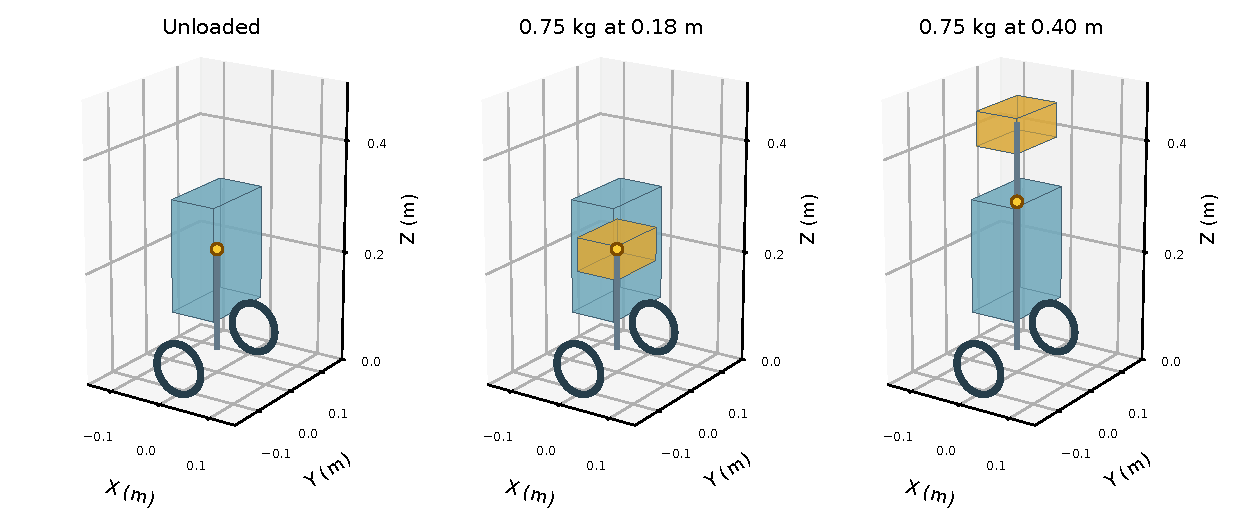
\includegraphics[width=\linewidth,height=.65\textheight,keepaspectratio]{../../figures/step4_fig07_payload_geometry.pdf}
\caption{Three-dimensional schematic at the upright pose, not a simulated response or a hardware design. Gold cuboid: payload; gold point: combined body COM; blue shell: illustrative original body envelope. Payload dimensions are those used for its pitch inertia. The original shell is only a drawing, and ballast may overlap its envelope. All three panels share the same metre scale. Dynamics remain planar, with no yaw, roll, slip or collision simulation.}
\end{figure}
The interactive lab now exposes payload mass and height alongside sensing settings. A gold cuboid shows the payload and the yellow point tracks the combined COM. The force arrow starts at that COM. The purple outline represents the estimated body and payload pose; changing load resets the run. JSON exports retain nominal and loaded parameters, load geometry, sensing settings, force events and trajectories. Recorded original experiments retain their original geometry and parameters.

\clearpage
\section*{6 Deterministic outcomes under a large push}
\begin{figure}[htbp]
\centering
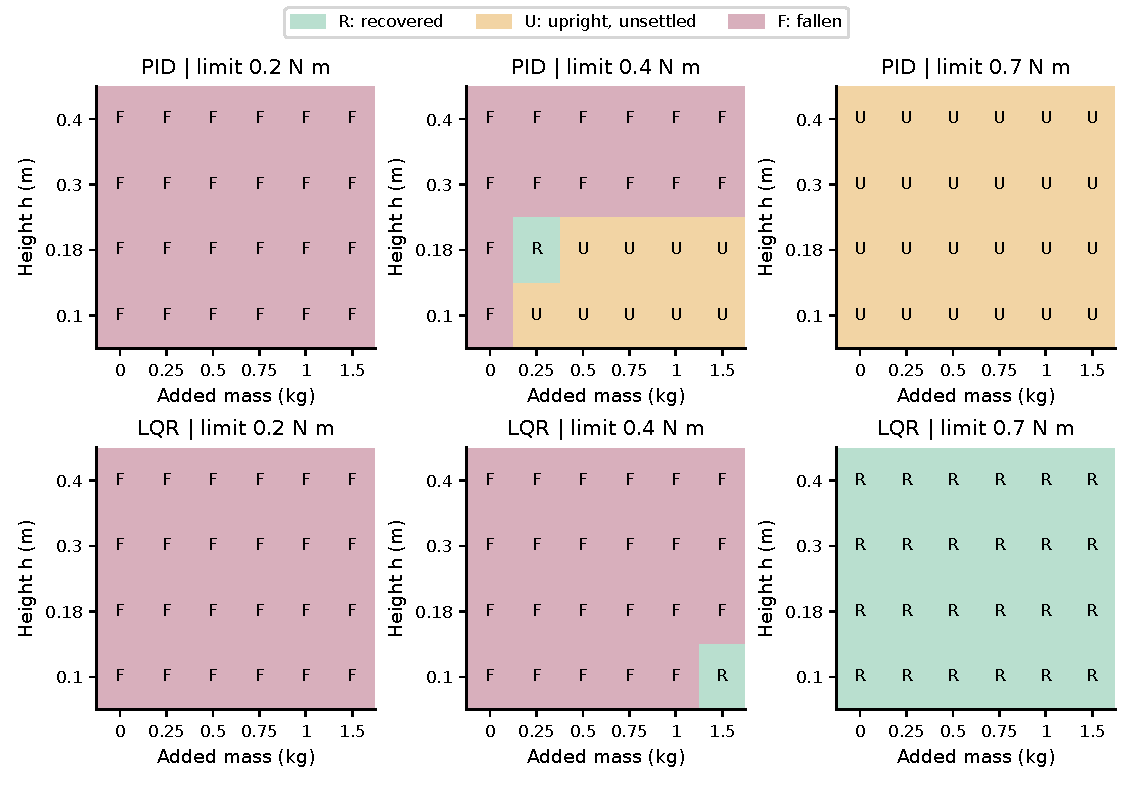
\includegraphics[width=\linewidth,height=.65\textheight,keepaspectratio]{../../figures/step4_fig02_outcome_map.pdf}
\caption{Deterministic outcomes for zero initial tilt and a 20 N pulse, separated by controller and torque limit. Each distinct loaded cell is one trial. The zero-mass column repeats the same unloaded trial across heights for reference; those repetitions are not additional trials. Masses and heights are discrete categories, not equally spaced numerical axes. These maps do not fit a stability boundary.}
\end{figure}
Read each cell as one evaluated condition. The outcomes reflect nonlinear response and saturation under frozen gains. The map deliberately retains both upright-but-unsettled and recovered states, because falling and position recovery answer different questions. It is not a load rating or a certified operating envelope.

\clearpage
\section*{7 Summaries over the common condition grid}
\begin{figure}[htbp]
\centering
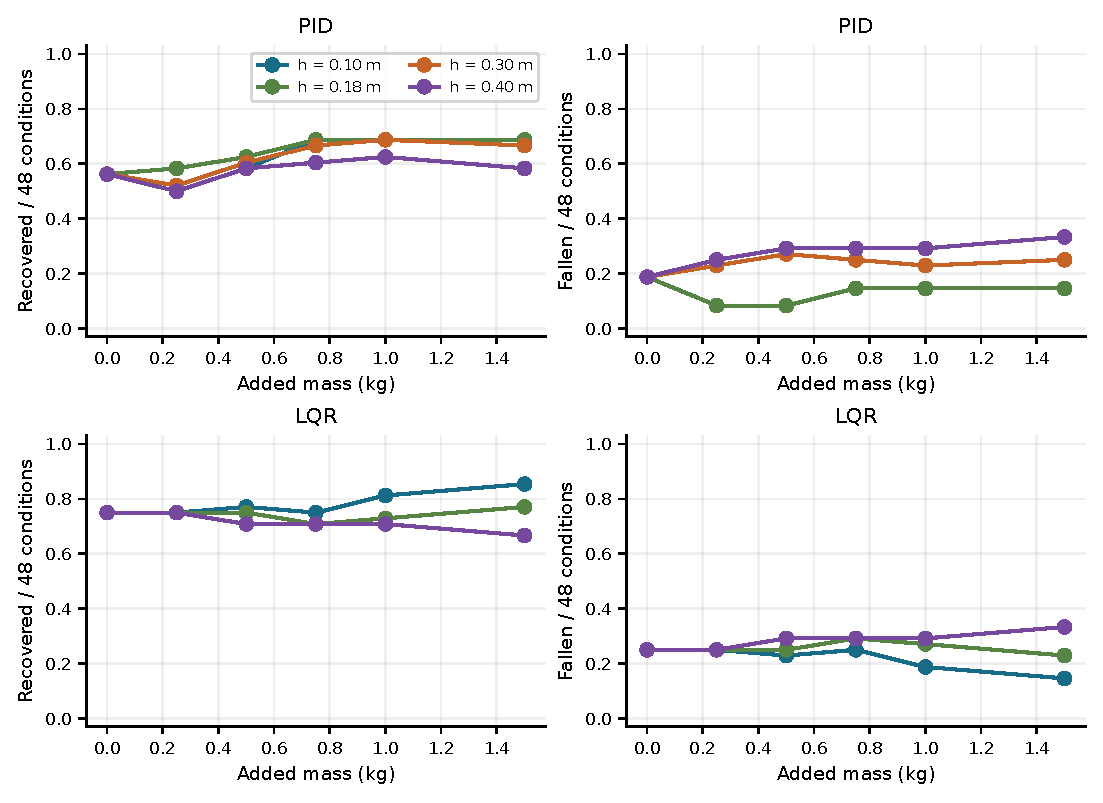
\includegraphics[width=\linewidth,height=.65\textheight,keepaspectratio]{../../figures/step4_fig03_grid_fractions.pdf}
\caption{Fractions of the same 48 deterministic initial-tilt/force/torque conditions at each load: four tilts, four force levels and three torque limits. The denominator includes zero-force cases. These equally weighted grid summaries are descriptive, not success probabilities for an operating population. No sampling confidence intervals apply. Lines only connect evaluated masses.}
\end{figure}
For each loaded case, ideal\_summary.csv also pairs its 48 outcomes with the same unloaded conditions. It records baseline-fall-to-upright and baseline-upright-to-fall transitions, so improvements and regressions can be inspected separately. Aggregate fractions can conceal which individual conditions changed. No claim of monotonic safety improvement, optimal mounting height or superiority of PID or LQR as a class is justified by this design.

\clearpage
\section*{8 Selected time responses}
\begin{figure}[htbp]
\centering
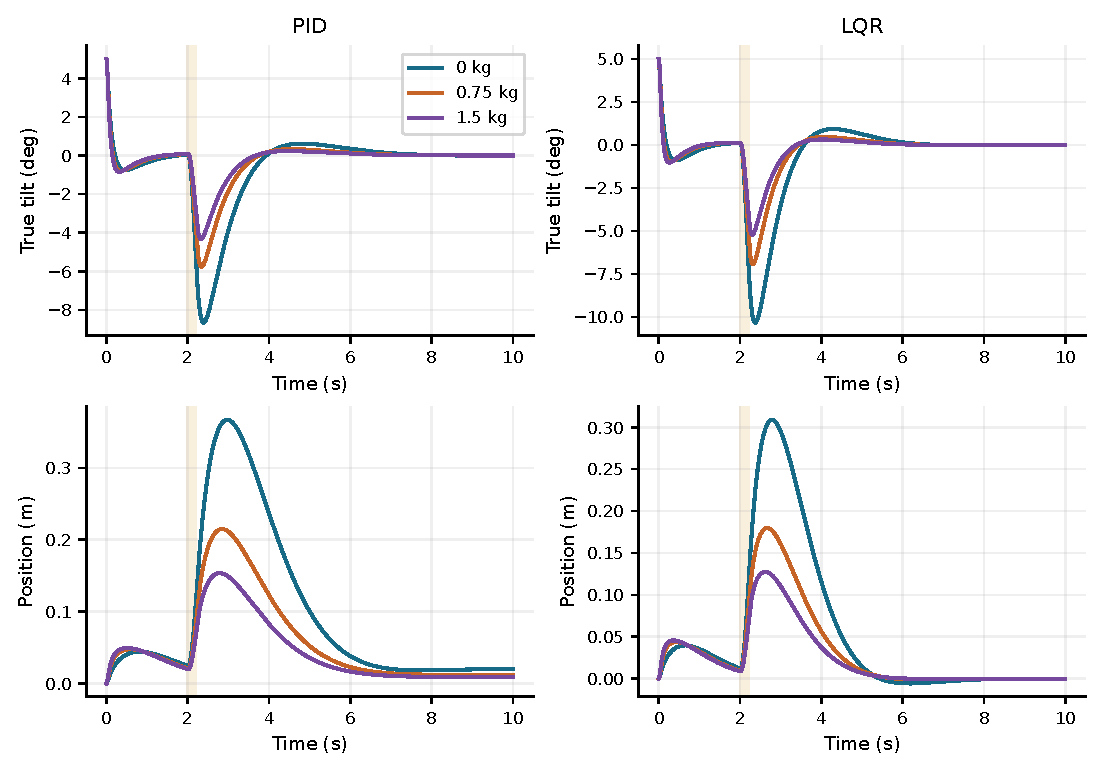
\includegraphics[width=\linewidth,height=.65\textheight,keepaspectratio]{../../figures/step4_fig04_trajectories.pdf}
\caption{Protocol-selected ideal-sensing examples: 5 deg initial tilt, 5 N pulse and 0.7 N m torque limit. Loaded examples mount their payload at h=0.40 m. The shaded interval is the pulse. All six trials last 10 s and recover. These traces illustrate one condition and do not establish that increasing payload always improves balance.}
\end{figure}
\textbf{Selected nominal examples, h=0.40 m when loaded}
\begin{longtable}{p{0.198\linewidth}p{0.216\linewidth}p{0.225\linewidth}p{0.261\linewidth}}
\toprule
Controller & Added mass (kg) & Peak tilt (deg) & Recovery after pulse (s) \\ \midrule \endhead
PID & 0 & 8.661 & 4.085 \\
PID & 0.75 & 5.766 & 3.440 \\
PID & 1.5 & 5.000 & 3.000 \\
LQR & 0 & 10.327 & 3.060 \\
LQR & 0.75 & 6.935 & 2.595 \\
LQR & 1.5 & 5.227 & 2.285 \\
\bottomrule
\end{longtable}
\clearpage
\section*{9 Loading combined with noisy sensing}
\begin{figure}[htbp]
\centering
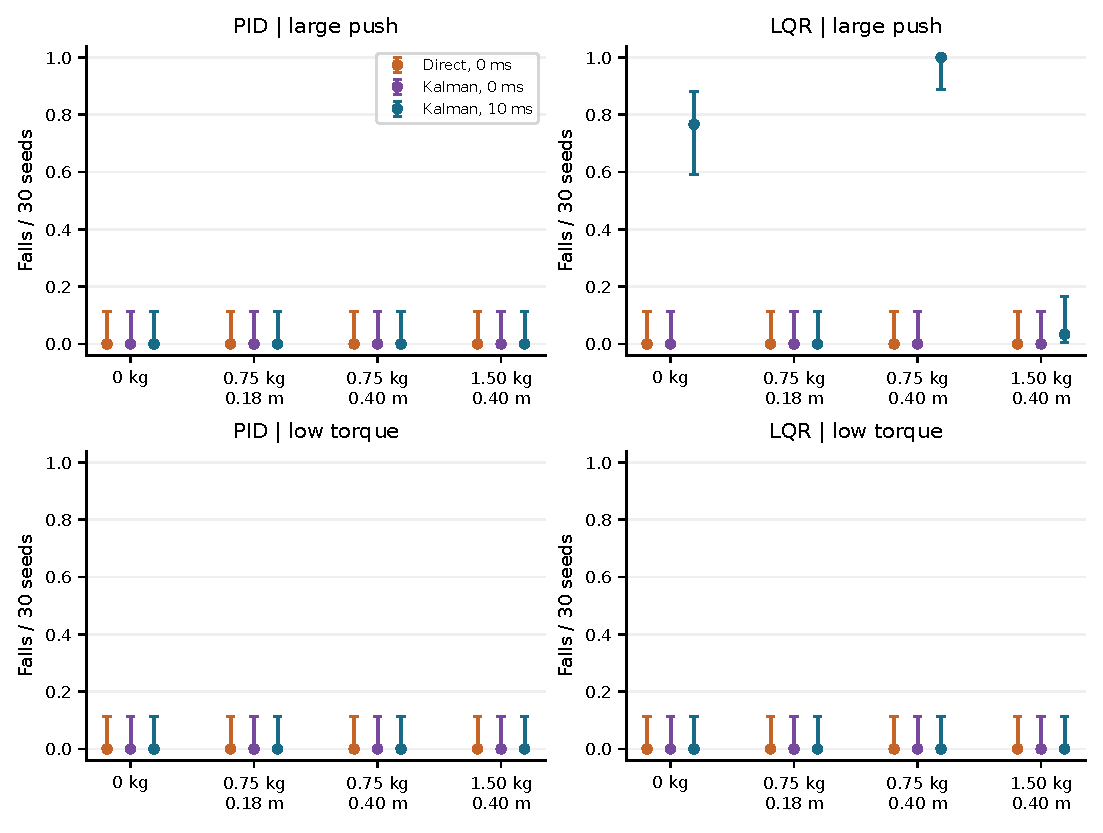
\includegraphics[width=\linewidth,height=.65\textheight,keepaspectratio]{../../figures/step4_fig05_sensing_falls.pdf}
\caption{Fall fractions and Wilson 95\% intervals for fixed noisy conditions. Each point uses 30 paired seeds, angle-noise SD 0.5 deg and gyro-noise SD 2 deg/s. The first load is the unloaded reference; labels for loaded cases give mass and mounting height. Large-push and low-torque scenarios retain their original definitions. Zero observed falls does not imply zero failure probability. Profiles share seeds and are not independent groups.}
\end{figure}
For LQR in the large-push scenario with Kalman sensing and 10 ms delay, falls are 23/30 unloaded, 0/30 at 0.75 kg and h=0.18 m, 30/30 at 0.75 kg and h=0.40 m, and 1/30 at 1.50 kg and h=0.40 m. This nonmonotone response is specific to those fixed conditions; more load is neither uniformly better nor uniformly worse.

This small sensing subset is a joint exploratory comparison, not a full mass-height-noise-delay factorial study. Noise may excite motion that is absent under exact state feedback. The filter smooths measurements at the delivered packet time; 10 ms delay remains uncompensated. Thirty seeds give limited resolution for uncommon failures. Zero observed falls in a cell has a Wilson upper bound of approximately 11.35\%.

\clearpage
\section*{10 Persistent motion among full-duration survivors}
\begin{figure}[htbp]
\centering
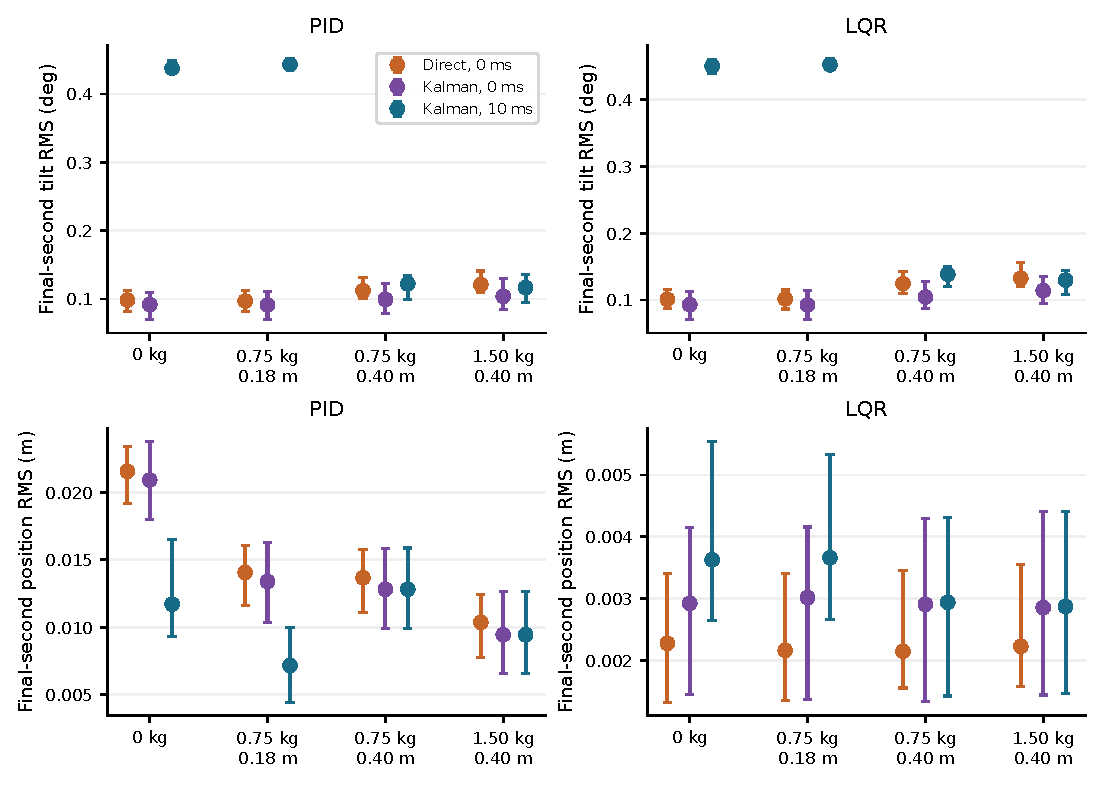
\includegraphics[width=\linewidth,height=.65\textheight,keepaspectratio]{../../figures/step4_fig06_tail_rms.pdf}
\caption{Nominal-condition final-one-second RMS metrics, sampled at 200 Hz including both endpoints from 9 to 10 s. Points show medians and bars the interquartile range across 30 seeds, not confidence intervals. Every plotted trial survives for 10 s but fails the strict continuous-dwell recovery criterion. These additional metrics describe persistent motion without redefining the recovery labels. Full-duration-only speed RMS is also supplied in the CSV.}
\end{figure}
The nominal sensing trials are all upright but unsettled. Tail RMS reveals differences hidden by that shared label without silently changing the original recovery criterion. A low RMS tilt alone does not guarantee low positional error or satisfy a continuous dwell condition. Tolerance choices should be tied to an eventual hardware task, then fixed before testing new controllers.

\clearpage
\section*{11 Verification, limitations and next experiments}
All 2,016 deterministic trials were repeated with two RK4 substeps per control interval, retaining the original 200 Hz sensing and controller update. 0 outcome labels changed. Numerical agreement of labels at this refinement does not prove global convergence or physical validity. Per-trial metric differences are retained in integration\_audit.json; the stochastic subset was not subjected to the full refinement audit.

Automated checks verify zero-payload trajectory parity, the component-wise inertia identity, a positive mass matrix over selected poses, no mutation of the nominal configuration, input bounds and repeatable seeded trials. A separate NumPy component mass-matrix calculation agrees with the JavaScript dynamics. Six selected loaded ideal trajectories also agree with the existing Python simulator. The 3D UI tests exercise resets, payload geometry, replay isolation and exports with a renderer mock. Browser access was unavailable, so interactive WebGL pixels were not visually verified.

The model omits wheel slip, roll, yaw, collisions, structural flexibility, motor electrical dynamics and hardware sensor calibration. Payload positions are centred, static and rigid; this study does not estimate an unknown payload, adapt gains, move a load online or compensate an off-axis equilibrium shift. The schematic shell is not a complete CAD mass distribution. Literature already studies unknown-payload estimation and physical wheeled-pendulum validation [2], so adding payload controls alone is not a research novelty claim.

The next defensible comparison is frozen gains versus a payload-aware redesign, with a declared tuning budget, separate development conditions and held-out mass-height/force combinations. A fixed attachment-point disturbance study would separate the effects of moving COM from the changing force moment. Independent simulator or hardware measurements should then test the chosen claims. Keep these supplements and their frozen datasets separate from the original manuscript until the author reviews the contribution, citations and AI-assistance disclosure.

\section*{Reproduction and files}
From the project root, run node run\_payload.js, then node run\_payload\_audit.js, then publication/.venv/Scripts/python.exe publication/build\_payload\_report.py. The protocol snapshot records settings and source hashes before execution. results/payload contains per-trial JSON/CSV, deterministic and sensing summaries, selected traces and the integration audit. Seven new figures are exported as vector PDF, SVG and 600 dpi PNG. The report is provided as HTML and PDF, with editable LaTeX source; LaTeX was not compiled here. The original manuscript and Step 3 datasets remain archived baselines.

\section*{References}
[1] MIT OpenCourseWare. Classical Mechanics, Fall 2016. Lesson 29.4: Parallel Axis Theorem. \url{https://ocw.mit.edu/courses/8-01sc-classical-mechanics-fall-2016/resources/29-3/}\par
[2] D. Baek, Y. Sim, A. Purushottam, S. Gupta and J. Ramos. Toward Control of Wheeled Humanoid Robots with Unknown Payloads: Equilibrium Point Estimation via Real-to-Sim Adaptation. arXiv:2403.10948v2, 2024. \url{https://arxiv.org/abs/2403.10948v2}\par
\end{document}
